\documentclass[pdf]{beamer}
%
% Choose how your presentation looks.
%
% For more themes, color themes and font themes, see:
% http://deic.uab.es/~iblanes/beamer_gallery/index_by_theme.html
%
\mode<presentation>
{
  \usetheme{AnnArbor}      % or try Darmstadt, Madrid, Warsaw, ...
  \usecolortheme{wolverine} % or try albatross, beaver, crane, ...
  \usefonttheme{default}  % or try serif, structurebold, ...
  \setbeamertemplate{navigation symbols}{}
  \setbeamertemplate{caption}[numbered]
} 

\usepackage[czech]{babel}
\usepackage[utf8]{inputenc}
\usepackage[T1]{fontenc}
\usepackage[lined,linesnumbered]{algorithm2e}
\usepackage[square,sort,comma,numbers]{natbib}

\title[ITY - 5. projekt]{Jarníkův algoritmus}
\author{Jan Zbořil, xzbori20}
\institute{FIT VUT Brno}
\date{\today}

\begin{document}

\begin{frame}
  \titlepage
\end{frame}

% Uncomment these lines for an automatically generated outline.
%\begin{frame}{Outline}
%  \tableofcontents
%\end{frame}

\section{O algoritmu}
\subsection{Úvod}

\begin{frame}{Jarníkův algoritmus}

\begin{itemize}
  \item<1-> v zahraničí jako Primův algoritmus
  \item<2-> hledá minimální kostru ohodnoceného grafu
\end{itemize}

\vskip 0.5cm

\begin{block}<3->{Co to znamená?}
Algoritmus najde takovou podmnožinu hran grafu, která tvoří strom obsahující všechny vrcholy původního grafu a součet ohodnocení hran z této množiny je minimální.
\end{block}

\end{frame}

\subsection{Pseudokód}
\begin{frame}{Pseudokód}
\begin{center}
    
\scalebox{.8}{                        %new code
    \begin{algorithm}[H]              %new code
        \DontPrintSemicolon
        \KwIn{vážený souvislý graf $(G,w)$}
        \For{each $x \in V(G)$}{
            $w(x) \leftarrow \infty $;
            $p(x) \leftarrow \perp $;
        }
        \texttt{Nepřipojené} = $V$; \\
        \While{\texttt{Nepřipojené} $\ne 0$}{
            Odeber z \texttt{Nepřipojené} vrchol $u$ s $w(u) =~$min$\{ w(x)~|~x \in V \}$;\\
            \For{each $\{u,u'\} \in E$}{
                \If{$u' \in \texttt{Nepřipojené} \wedge w(u') \textless w(\{u,u'\})$}{
                    $w(u') \leftarrow w(\{u,u'\})$;
                    $p(u') \leftarrow u$;
                }
            }
        }
    \end{algorithm}
}
\end{center}
\begin{itemize}
    \item Na konci je $T = (V, \{\{ p(u),u \}~|~u \in V,~p(u) \ne \perp \})$ minimální kostra $(G,w)$.
\end{itemize}

\end{frame}

%%%%%%%%%%%%%%%% NOVY SNIMEK %%%%%%%%%%%%%%%%
\subsection{Časová složitost}
\begin{frame}{Časová složitost}

\begin{itemize}
\item<1-> Každý vrchol je připojen právě jednou, a v té chvíli jsou zpracovány všechny jeho hrany.
\item<2->  Každá hrana má dva konce, proto je testována dvakrát.
\item<3->  Dodatečný čas je potřeba k výběrům minima na řádku 6 (možno v logaritmickém čase k počtu vrcholů).
\item<4->  Potřebný čas je maximálně přímo úměrný $ |E| \log_2|V| $.
\item<5->  Následující tabulka ukazuje časovou složitost dle zvolené implementace
\end{itemize}

% Commands to include a figure:
%\begin{figure}
%\includegraphics[width=\textwidth]{your-figure's-file-name}
%\caption{\label{fig:your-figure}Caption goes here.}
%\end{figure}

\small
\onslide<6->
\begin{table}
\centering
\begin{tabular}{| l | l |}
\hline
\textbf{Datová struktura s ohodnocením hran} & \textbf{Celková časová složitost}\\\hline
matice sousednosti & $V^2$ \\
binární halda a seznam sousedů & $O((V+E))\log(V)=E \log (V)$ \\
Fibonacciho halda a seznam sousedů & $E+V\log(V)$ \\
\hline
\end{tabular}
\caption{\label{tab:widgets}časová složitost Jarníkova algoritmu.}
\end{table}

\end{frame}

\normalsize
\section{Příklad}
\begin{centering}
\begin{frame}{Příklad algoritmu}
    \begin{onlyenv}<1>
        \begin{figure}[h!]
        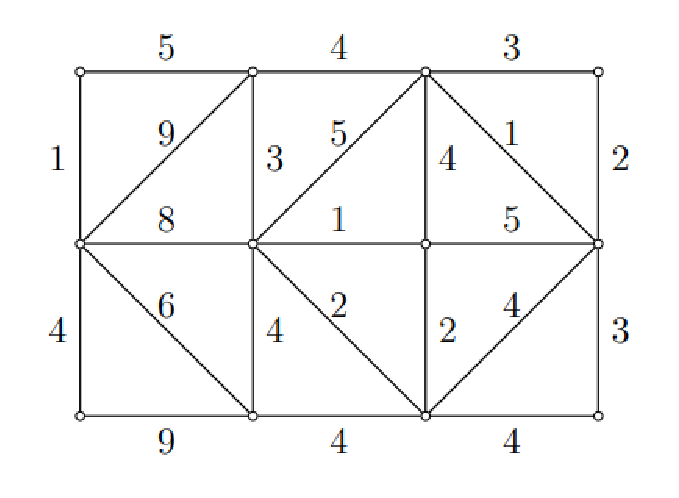
\includegraphics[scale=0.5]{obr1.eps}
        \caption{\label{fig:obr1}stav před aplikací algoritmu}
        \end{figure}
    \end{onlyenv}
    
    \begin{onlyenv}<2>
        \begin{figure}[h!]
        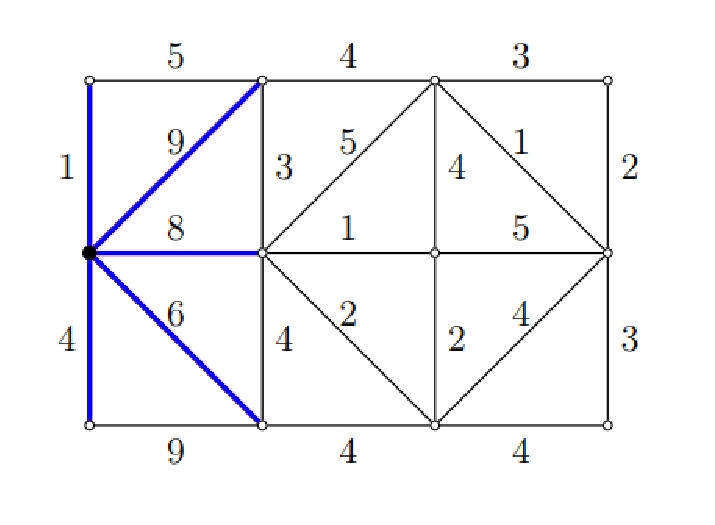
\includegraphics[scale=0.5]{obr2.eps}
        \caption{\label{fig:obr2}počáteční bod}
        \end{figure}
    \end{onlyenv}
    
    \begin{onlyenv}<3>
        \begin{figure}[h!]
        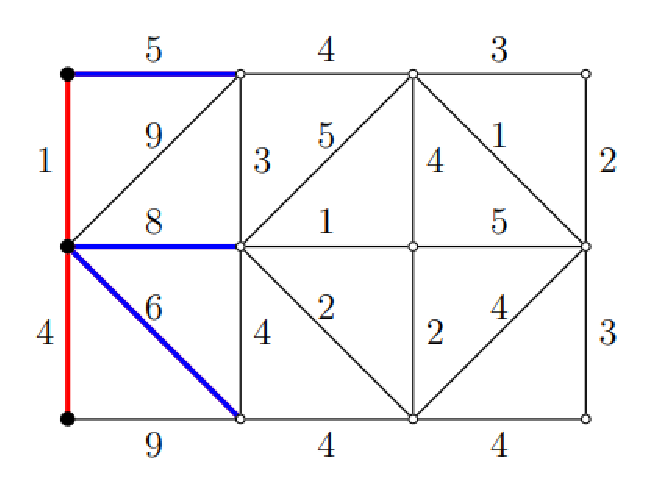
\includegraphics[scale=0.5]{obr3.eps}
        \caption{\label{fig:obr}výběr nejkratší cesty s váhou 1 a 4 a nejkratší cesty do bodu původně spojeného cestou 9, nyní 1+5}
        \end{figure}
    \end{onlyenv}
    
    \begin{onlyenv}<4>
        \begin{figure}[h!]
        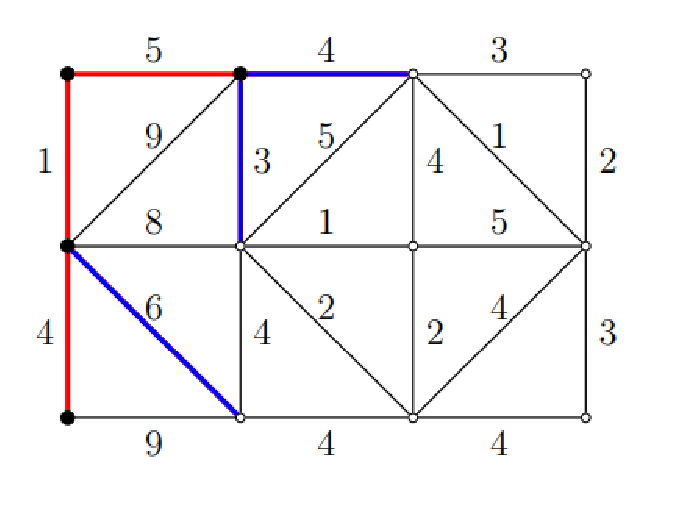
\includegraphics[scale=0.5]{obr4.eps}
        \caption{\label{fig:obr4}přidání cesty 1+5+4 a změna z 8 na 1+5+3}
        \end{figure}
    \end{onlyenv}
    
    \begin{onlyenv}<5>
        \begin{figure}[h!]
        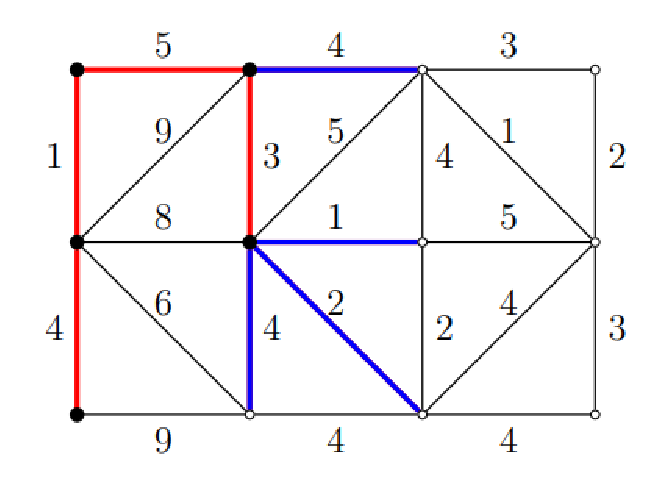
\includegraphics[scale=0.5]{obr5.eps}
        \caption{\label{fig:obr5}přidání bodu 1+5+4+1 a 1+5+4+1+2, změna cesty z 6 na 1+5+3+4, protože 4 \textless~6}
        \end{figure}
    \end{onlyenv}
    
    \begin{onlyenv}<6>
        \begin{figure}[h!]
        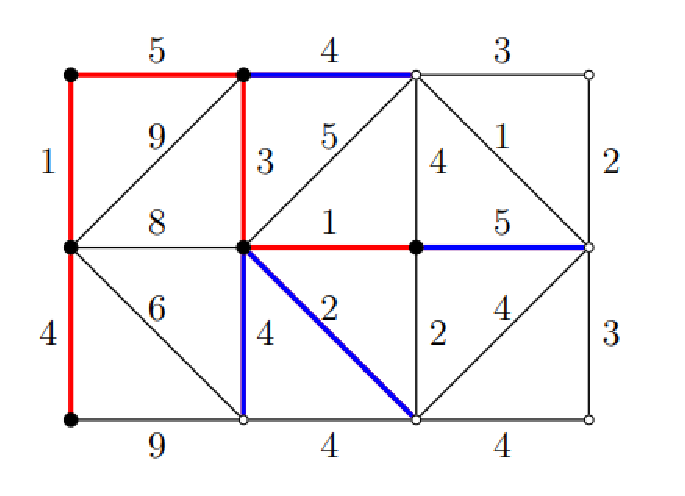
\includegraphics[scale=0.5]{obr6.eps}
        \caption{\label{fig:obr6}výběr cesty 1+5+3+1, přidání bodu 1+5+3+1+5}
        \end{figure}
    \end{onlyenv}
    
    \begin{onlyenv}<7>
        \begin{figure}[h!]
        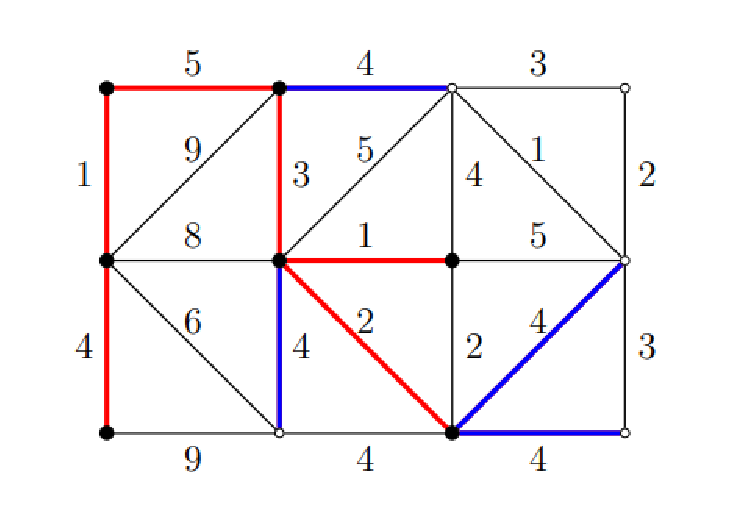
\includegraphics[scale=0.5]{obr7.eps}
        \caption{\label{fig:obr7}výběr cesty 1+5+3+2, přidání bodu 1+5+3+2+4 a 1+5+3+2+4}
        \end{figure}
    \end{onlyenv}
    
    \begin{onlyenv}<8>
        \begin{figure}[h!]
        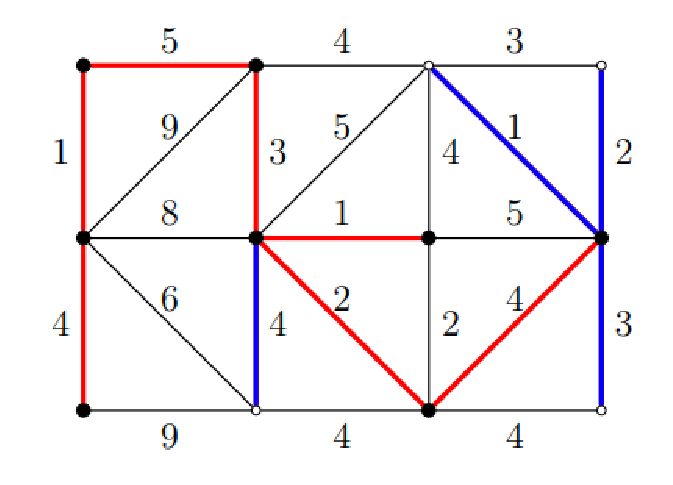
\includegraphics[scale=0.5]{obr8.eps}
        \caption{\label{fig:obr8}výběr cesty 1+5+3+2+4, přidání bodů 1+5+3+2+4+1, 1+5+3+2+4+2 a 1+5+3+2+4+3, odstranění 1+5+4, protože 1 \textless~4}
        \end{figure}
    \end{onlyenv}
    
    \begin{onlyenv}<9>
        \begin{figure}[h!]
        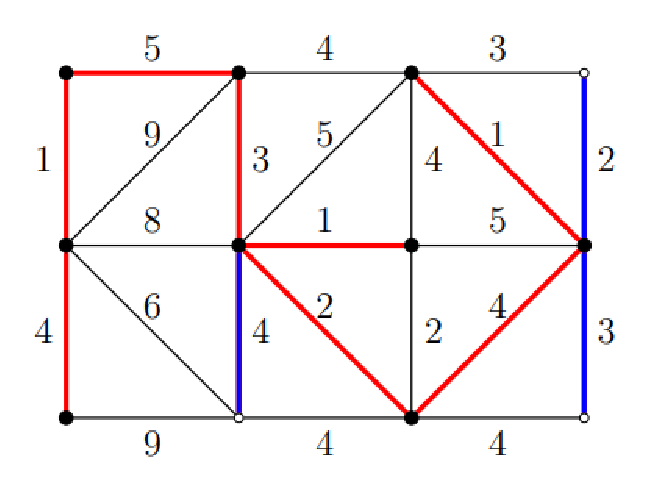
\includegraphics[scale=0.5]{obr9.eps}
        \caption{\label{fig:obr9}výběr nejkratší cesty 1+5+3+2+4+1}
        \end{figure}
    \end{onlyenv}
    
    \begin{onlyenv}<10>
        \begin{figure}[h!]
        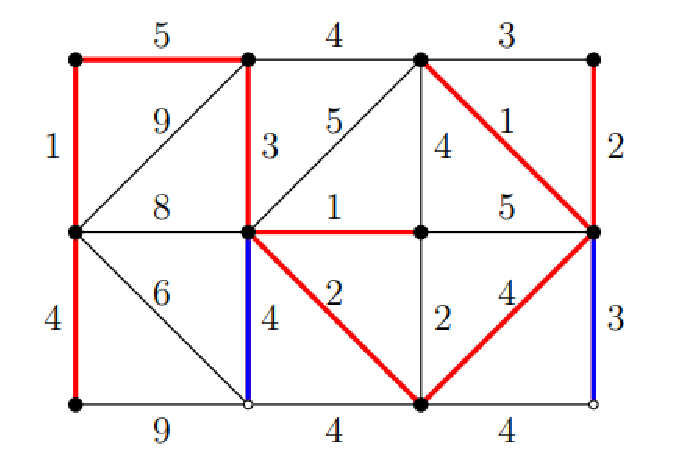
\includegraphics[scale=0.5]{obr10.eps}
        \caption{\label{fig:obr10}výběr nejkratší cesty 1+5+3+2+4+2}
        \end{figure}
    \end{onlyenv}
    
    \begin{onlyenv}<11>
        \begin{figure}[h!]
        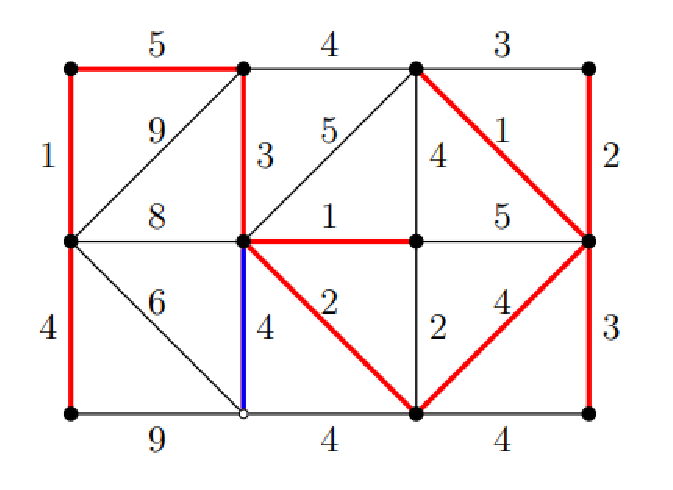
\includegraphics[scale=0.5]{obr11.eps}
        \caption{\label{fig:obr11}výběr nejkratší cesty 1+5+3+2+4+3}
        \end{figure}
    \end{onlyenv}
    
    \begin{onlyenv}<12>
        \begin{figure}[h!]
        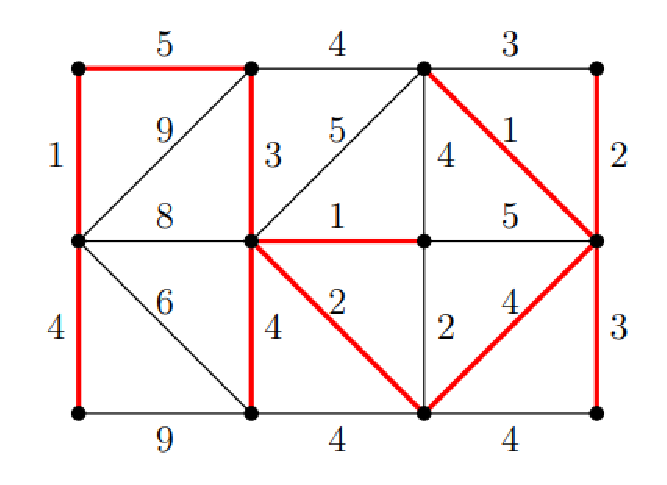
\includegraphics[scale=0.5]{obr12.eps}
        \caption{\label{fig:obr12}výběr nejkratší cesty 1+5+3+4}
        \end{figure}
        Algoritmus nyní skončil, protože všechny bodu grafu jsou spojené minimální kostrou.    \end{onlyenv}

\end{frame}
\end{centering}  

\section{Zdroje}
\begin{frame}{Zdroje}
    \begin{thebibliography}{99}
    
        \bibitem{Lengal} O. Lengál. Teorie grafu. [online], Brno, CZ: FIT VUT, 2019. Zobrazeno 23. 3. 2020. Dostupné na: http://www.fit.vutbr.cz/~lengal/idm/grafy-algoritmy.pdf

         \bibitem{wiki} Wikipedia contributors. Jarníkův algoritmus --- Wikipedie. [online], 2004. Zobrazeno 23. 3. 2020. Dostupné na: https://cs.wikipedia.org/wiki/Jarníkův\_algoritmus
        
    \end{thebibliography}
\end{frame}

    
\end{document}
